\section{Proposed Method}
Given a trained DNN classifier $\bff$ and a paired OOD detector $\calD_\gamma$, our goal is to learn a set of concepts that can provide explanations for the predictions of the detector.
We first propose new metrics for quantifying the set of learned concepts, followed by a general framework for learning the concepts.
% This section explains our evaluation metrics and methods: (1) how to gauge the utility of a given set of concepts for OOD detector explanation, and (2) a general learning algorithm to discover concepts that \jihye{incomplete yet}

\mypara{ID and OOD Datasets.}
% Throughout the paper, 
We assume the availability of a labeled ID training dataset $\Dintr = \{(\bfx_i, y_i), ~i = 1, \cdots, \Nintr\}$ from the distribution $\Pin$, where $y_i \in \outputs$ is the class label for an input $\bfx_i \in \inputs$.
We also assume the availability of an unlabeled training dataset $\Douttr = \{\widetilde{\bfx}_i, ~i = 1, \cdots,  \Nouttr\}$ from a different distribution, referred to as the {\em auxiliary OOD dataset}.
Similarly, we define the ID validation and test datasets (sampled from $\Pin$) as $\Dinval$ and $\Dinte$, and the OOD validation and test datasets as $\Doutval$ and $\Doutte$.
We note that the auxiliary OOD dataset $\Dintr$ and validation OOD dataset $\Dinval$ are sampled from the same auxiliary distribution (\eg the MS-COCO dataset). However, the test OOD dataset can be from an entirely different and unknown distribution (\eg the SUN dataset), as is often the case in reality.
% Add notation for the number of samples if needed.
All the OOD datasets are unlabeled since their label space can be different from $\outputs$. One can think of the OOD datasets for training, validation, and test to be biased samples from an unknown OOD marginal distribution $\Pout(\bfx)$.

\mypara{Concept Scores.}
We start by formalizing how to compute a representative score for concepts given an input, which will be used for evaluation in Section \ref{sec:completeness_score} and Section \ref{sec:separability_score}.
A projection matrix $\bfC \in \reals^{d_\ell \times m}$ that maps $\bfphi(\bfx)$ to $\bfv_{\bfC}(\bfx)$ consists of $m$ unit (column) vectors $\,\bfC := [\bfc_1 \cdots \bfc_m]$, where each $\bfc_i$ is referred to as a \textit{concept vector} representing the $i$-th concept (\eg "stripe", "oval face", etc.), and $m$ is the number of concepts.
The inner product between the feature representation and a concept vector quantifies how close the input is to the given concept, and this is referred to as the concept score. 
Specifically, the concept score correicsponding to concept $i$ is $\bfv_{\bfc_i}(\bfx) = \langle \bfphi(\bfx), \bfc_i \rangle \in \reals^{a_\ell b_\ell}$, which is the $a_\ell \times b_\ell$ times concatenation over the standard inner-products (between vectors) $\,\langle \bfphi^{p,q}(\bfx), \bfc_i \rangle \in \reals, ~\forall p, q \in [a_\ell] \times [b_\ell]$, where $\bfphi^{p,q}$ is the feature representation corresponding to the $(p, q)$-th patch of input $\bfx$ (\ie receptive field).
That is, $\bfv_{\bfc_i}(\bfx)$ \ryan{maybe $\bfv_{\bfc_i}^{(p,q)}(\bfx)?$} is the concept score of $(p, q)$-th patch of $\bfx$ with respect to $i$-th concept, and if it is a large positive (or negative) value, then the corresponding part of input is positively (or negatively) aligned with the concept.
The vector of concept scores from all the concepts is defined simply as the concatenation of the individual concept scores, \ie $\VC(\bfx)^T = [\bfv_{\bfc_1}(\bfx)^T, \cdots, \bfv_{\bfc_m}(\bfx)^T] \in \reals^{a_\ell b_\ell m}$.

% When $p = q = 1$ for fully-connected layers (\ie the receptive field of $\bfphi$ corresponds to the entire input $\bfx_i$), $\langle \bfphi(\bfx_i),~\bfc_j \rangle$ is a scalar concept score that represents the input.
% On the other hand, when $p, q > 1$, to obtain a scalar concept score for a given input, we take the maximum absolute concept score across the $p \times q$ patches, corresponding to $p \times q$ feature representations.
% To define the overall closeness of an input $\bfx_i$ and the concept $\bfc_j$ with a scalar concept score, we take the maximum absolute concept score across the $p \times q$ patches of $\bfx_i$.
When $p, q > 1$ (unless a fully-connected layer is of interest), where the receptive field of $\bfphi$ corresponds to the entire input $\bfx_i$), we also define a dimension-reduced version of the concept score vector that takes the maximum of the inner-product over each $a_\ell \times b_\ell$ patch (instead of concatenating them) as follows: $\TVC(\bfx)^T = [\widetilde{v}_{\bfc_1}(\bfx), \cdots, \widetilde{v}_{\bfc_m}(\bfx)] \in \reals^m$, where $\widetilde{v}_{\bfc_i}(\bfx) = \max_{p, q} |\langle \bfphi^{p,q}(\bfx), \bfc_i \rangle| \in \reals$.
% The intuition behind taking a maximum score across the patches of input is as follows.
This reduction operation is done to capture the most important correlations from each patch.
Suppose $\bfc_j$ represents a striped pattern and $\bfx_i$ is an image of a zebra standing on grass.
The patch of greenery background should get a low concept score, while a patch of the zebra's body should get high concept score.
% As the defining score for the stripe concept, we decide to take the score from the patch of zebra's body, out of all patches constituting the entire input image.
Out of all the patches constituting the input image, we take the maximum score (likely) corresponding to a patch of the zebra's body as the defining score for the striped concept.

Based on the concept scores and data defined as above, we elaborate the evaluation criteria of concepts for the purpose of OOD detector explanation in Section \ref{sec:completeness_score} and Section \ref{sec:separability_score}, followed by a general learning algorithm to discover concepts that satisfy the criteria in Section \ref{sec:concept_learning}.

\subsection{Completeness Score for Concepts}
\label{sec:completeness_score}
In this subsection, we address the following questions \ryan{: 1) are the set of learned concepts $\bfC$ sufficient to similarly match the behavior of the original classifier $\bff$ and 2) are the set of learned concepts $\bfC$ sufficient to similarly match the behavior of the OOD detector $\calD$? Such properties would indicate that the concepts learned are appropriate for describing the behavior of $\bfC$ and $\calD$. }: \textit{}
\jihye{yes, I'm still working on this paragraph}

% Given a trained DNN classifier $\bff$ and a trained OOD detector $\calD_\gamma$, our goal is to learn a set of concepts that can provide explanations for the predictions of the classifier and detector.
% To this end, we first propose new metrics for quantifying a set of learned concepts, followed by a general framework for learning a set of concepts.


Given a sufficient set of concepts $\bfC$, the classifier in the concept world should be able to closely approximate the prediction performance of the original classifier.
Likewise, the detector in the concept world should be able to closely approximate the detection performance of the original detector.
In order to concretely quantify this notion, we next define a 
completeness score for the set of concepts with respect to the classification task and the OOD detection task.

\begin{definition}
\label{def:completeness_class}
Given a trained DNN classifier $\bff = \bfh \circ \bfphi\,$ and a set of concept vectors $\bfC$, the {\em classification completeness score} with respect to an ID distribution $\Pin(\bfx, y)$ is defined as in \cite{yeh2019completeness}:
\begin{align}
\label{equ: completeness-classification}
    &\eta^{}_\bff(\bfC) ~:= \\ 
    &\frac{\textrm{sup}_\bfg \,\expec_{(\bfx, y) \sim \Pin} \indicator[ y = \argmax_{y'} h_{y'}(\recphi(\bfx)) ] ~-~ a_r}{\expec_{(\bfx, y) \sim \Pin} \indicator[y = \argmax_{y'} h_{y'}(\bfphi(\bfx))] ~-~ a_r} \nonumber
\end{align}
where $a_r$ is the accuracy of random prediction (\ie $a_r = 1/L$ for $L$ classes).
\end{definition}
In the numerator, the maximization is over the parameters of the fully-connected neural network $\bfg$ that reconstructs the feature representation from the vector of concept scores \jihye{is this sentence necessary?}.
The denominator of $\eta^{}_\bff(\bfC)$ is the accuracy of the classifier $\bff$ in canonical world, while the numerator is the maximum accuracy that can be achieved using the feature representation reconstructed from the concept-score vector in concept world.
In practice, the expectation is estimated using a held-out test dataset $\Dinte$ from the ID distribution.

% \jihye{Limitation of the above completeness for our purpose. Need for / intuition behind detection completeness. fig (\ref{fig:detection-completeness})} \\.\\.\\.\\.\\.
% \jihye{Full elaboration on the two-world game -- fig \ref{fig:detection-completeness}}

\begin{definition}
\label{def:completeness_detec}
Given a trained DNN classifier $\bff = \bfh \circ \bfphi$, a trained OOD detector with score function $S(\bfx, \bff)$, and a set of concept vectors $\bfC$, the {\em detection completeness score} with respect to ID distribution $\Pin(\bfx, y)$ and OOD distribution $\Pout(\bfx)$ is defined as
\begin{align}
\label{equ: completeness-detection}
    \eta^{}_{\bff, S}(\bfC) 
    ~:=~ \frac{\textrm{sup}_\bfg \,\textrm{AUC}(\bfh \circ \recphi) ~-~ b_r}{\textrm{AUC}(\bfh \circ \bfphi) ~-~ b_r},
\end{align}
% where $\recphi(\bfx) = \bfg(\bfv_{\bfC}(\bfx))$ is the feature representation reconstructed from the concept scores, 
where $\textrm{AUC}(\bff)$ is the area under the ROC curve of an OOD detector for $\bff$, defined as
\begin{align}
\label{equ:auroc_ideal}
\textrm{AUC}(\bff) ~:= \!\!\expec_{(\bfx, y) \sim \Pin} \expec_{\,\bfx^\prime \sim \Pout} \indicator\big[ S(\bfx, \bff) \,>\, S(\bfx^\prime, \bff) \big],
\end{align}
and $b_r = 0.5$ is the AUROC of a random detector.
\end{definition}
As with the classification completeness, the maximization in the numerator is over the parameters of the fully-connected network $\bfg$ that reconstructs the feature representation from the vector of concept scores \jihye{is this sentence necessary?}.
In practice, $\textrm{AUC}(\bff)$ is estimated using held-out test datasets from both the ID and OOD. Given an ID test dataset $\Dinte$ and an OOD test dataset $\Doutte$, the sample estimate of $\textrm{AUC}(\bff)$ is given by
\begin{align*}
    \widehat{\textrm{AUC}}(\bff) \,=\, \frac{1}{|\Dinte|\,|\Doutte|} \!\!\mysum_{(\bfx, y) \in \Dinte} \mysum_{~\bfx^\prime \in \Doutte} \!\!\!\indicator\big[ S(\bfx, \bff) > S(\bfx^\prime, \bff) \big]. 
\end{align*}

Both the classification completeness and detection completeness scores have a range $[0, 1]$ \jihye{technically, $> 1$ is possible} \ryan{probably worth explaining how this can happen}, and a value close to $1$ indicates that the set of concepts $\bfC$ are close to complete in characterizing the behavior of the classifier and/or the OOD detector.

\subsection{Concept Separability Score}
\label{sec:separability_score}
\iffalse

% \somesh{Assumptions: enforcing separability of each individual separability --> anyway leads to better separability with combined concepts}
% \somesh{First describe the problem -what we want to do. There are these possible methods..... We chose this because of what. It should never appear like magic.}
% \somesh{Some curve -- accuracy vs separability something like that}

\jihye{need for/intuition behind separablility. Full elaboration on the idea behind separability in concept space -- fig \ref{fig:detection-separability}.} Other than the completeness scores of Eq. (\ref{equ: completeness-classification}) and Eq. (\ref{equ: completeness-detection}), we also want the concept scores between ID and OOD data to be easily distinguishable. This notion is captured by the \textit{separability} metric in Eq. (\ref{equ: distinguishability}). 


An important property that we would like to impose on the set of learned concepts for the OOD detection task is that the ID data and OOD data be well separated in the dimension-reduced concept-score space.
The motivation behind this requirement is two-fold.
The first is that we would like the concept scores to be highly distinguishable between the ID and OOD data (\eg Fig.~\ref{fig:detection-separability}), in order to effectively interpret the detector's decisions.
The second is that we would like the detector in the concept world Eq. (\ref{equ:detector_concept}) to have performance close to that of the original detector, which requires that the distribution of detector scores $\Scon(\cdot)$ from ID and OOD data be well separated.
% maybe we should say requirement of high detection completeness here?
This in-turn translates to a requirement of good separability (between ID and OOD) in the projected concept-score space.
\fi

;Formally, we would like the set of concept-score vectors from the ID class $\,V_{\textrm{in}}(\bfC) := \{\TVC(\bfx) \in \reals^m ~:~ \bfx \sim \Pin\}$ and set of concept-score vectors from the OOD class $\,V_{\textrm{out}}(\bfC) := \{\TVC(\bfx) \in \reals^m ~:~ \bfx \sim \Pout\}$ to be well separated \ryan{to help ensure clear distinctions in the explanations between ID and OOD}.
Let $\,J_{\textrm{sep}}(V_{\textrm{in}}(\bfC), V_{\textrm{out}}(\bfC)) \in \reals$ define a general {\it measure of separability} between the two data subsets, such that a larger value corresponds to higher separability.
We will discuss specific choices for $J_{\textrm{sep}}$ that make it possible to tractable optimize the concept separability as part of the learning objective.

Class separability metrics have been well studied in the pattern recognition literature, particularly for the two-class case~\cite{fukunaga1990separ}~\footnote{Note that the two classes correspond to ID and OOD data.}. 
Distributional divergences such as the Kullback-Leibler and Hellinger distance can be used when the probability distribution of the two classes are known, and the divergence is tractable to compute.
Non-parametric measures of class separability (\eg based on $k$-nearest neighbors) are also candidates here, but they are usually hard to optimize using gradient-based methods.
In order to obtain a closed-form expression for the class separability, it is common to make simplifying assumptions on the class-conditional density (\eg multivariate Gaussian per class).
% We next propose a binary class separability 

\mypara{Global Concept Separability.}
Motivated by Fisher's linear discriminant analysis (LDA), we explore the use of class-separability measures based on the within-class and between-class scatter matrices~\cite{murphy2012separ}.
The goal of LDA is to find a projection vector (direction) such that data from the two classes are maximally separated and form compact clusters when projected onto this vector. 
Rather than finding an optimal projection direction, we are more interested in ensuring that the concept-score vectors from the ID and OOD data have high separability.
Given the set of concept-score vectors from the ID data $V_{\textrm{in}}(\bfC)$ and OOD data $V_{\textrm{out}}(\bfC)$, consider their within-class and between-class scatter matrices defined as
\begin{align}
\label{eq:scatter_matrices}
\bfS_w ~&= \mysum_{\bfv \in V_{\textrm{in}}(\bfC)} (\bfv \,-\, \bfmu_{\textrm{in}})\,(\bfv \,-\, \bfmu_{\textrm{in}})^T \nonumber \\
&+ \mysum_{\bfv \in V_{\textrm{out}}(\bfC)} (\bfv \,-\, \bfmu_{\textrm{out}})\,(\bfv \,-\, \bfmu_{\textrm{out}})^T, \\
%
\bfS_b ~&=~ (\bfmu_{\textrm{out}} \,-\, \bfmu_{\textrm{in}})\,(\bfmu_{\textrm{out}} \,-\, \bfmu_{\textrm{in}})^T,
\end{align}
where $\bfmu_{\textrm{in}}$ and $\bfmu_{\textrm{out}}$ are the mean concept-score vectors corresponding to the ID and OOD data respectively.
We define the following separability metric between based on the generalized eigenvalue equation solved by Fisher's LDA~\cite{fukunaga1990separ, murphy2012separ}:
\begin{align}
\label{eq:separability_trace}
&J_{\textrm{sep}}(V_{\textrm{in}}(\bfC), V_{\textrm{out}}(\bfC)) ~=~ \textrm{tr}\big[\bfS_w^{-1} \,\bfS_b\big] \nonumber \\
% &=~ \textrm{tr}\big[\bfS_w^{-1} \,(\bfmu_{\textrm{out}} \,-\, \bfmu_{\textrm{in}})\,(\bfmu_{\textrm{out}} \,-\, \bfmu_{\textrm{in}})^T\big] \nonumber \\
&=~ (\bfmu_{\textrm{out}} \,-\, \bfmu_{\textrm{in}})^T \,\bfS_w^{-1} \,(\bfmu_{\textrm{out}} \,-\, \bfmu_{\textrm{in}}).
\end{align}
Maximizing the above metric is equivalent to maximizing the sum of eigenvalues of the matrix $\,\bfS_w^{-1} \,\bfS_b$, which in-turn ensures a large between-class separability and a small within-class separability for the ID and OOD concept scores.
We refer to this as a {\em global concept separability} metric because it does not analyze the separability between the ID and OOD data on a per-class level.
% it analyzes the ID and OOD data from all the $L$ classes.

\jihye{Check if the motivation for "multivariate" separability is conveyed here.}

\mypara{Connection to the Bhattacharya distance.}
We note that the separability metric in Eq. (\ref{eq:separability_trace}) is closely related to the Bhattacharya distance~\cite{bhattacharyya1943measure} for the special case when the concept scores from both ID and OOD data follow a multivariate Gaussian density. The Bhattacharya distance is a well known measure of divergence between two probability distributions, and it has the nice property of being an upper bound to the Bayes error rate in the two-class case~\cite{fukunaga1990bhatta}. For the special case when the concept scores from both ID and OOD data follow a multivariate Gaussian with a shared covariance matrix, it can be shown that the Bhattacharya distance reduces to the separability metric in Eq. (\ref{eq:separability_trace}) (ignoring scale factors). 

\iffalse

We sometimes denote $J_{\textrm{sep}}(V_{\textrm{in}}(\bfC), V_{\textrm{out}}(\bfC))$ as $J_{\textrm{sep}}(\bfC)$ for brevity.
Assumption of unimodal distribution; when this assumption may not be appropriate in some cases. 

\fi


\mypara{Per-Class Concept Separability.}
% Conditioned on a given predicted class
So far, we have focused on the separability between the concept scores of ID and OOD data without considering the class prediction of the classifier.
However, it may be more appropriate to impose high separability between the concept scores on a per-class level. In other words, we would like the concept scores of ID and OOD data predicted by the classifier into any given class $y \in [L]$ to be well separated.
Consider the set of concept-score vectors from ID data that are predicted into class $y$: $V^{y}_{\textrm{in}}(\bfC) := \{\TVC(\bfx) \in \reals^m ~:~ \bfx \sim \Pin, ~\widehat{y}(\bfx) = y\}$. 
Likewise, define for the OOD data $\,V^{y}_{\textrm{out}}(\bfC) := \{\TVC(\bfx) \in \reals^m ~:~ \bfx \sim \Pout, ~\widehat{y}(\bfx) = y\}$. 
We can extend the definition of the separability metric for a given predicted class $y \in [L]$ as follows
\begin{align}
\label{eq:separability_trace_per_class}
&J_{\textrm{sep}}(V^{y}_{\textrm{in}}(\bfC), V^{y}_{\textrm{out}}(\bfC)) ~=~ \textrm{tr}\big[(\bfS^{y}_w)^{-1} \,\bfS^y_b\big] \nonumber \\
&=~ (\bfmu^y_{\textrm{out}} \,-\, \bfmu^y_{\textrm{in}})^T \,(\bfS^y_w)^{-1} \,(\bfmu^y_{\textrm{out}} \,-\, \bfmu^y_{\textrm{in}}).
\end{align}
The scatter matrices $\bfS^y_w$ and $\bfS^y_b$ are defined similar to Eq. (\ref{eq:scatter_matrices}), using the per-class subset of concept scores $V^{y}_{\textrm{in}}(\bfC)$ or $V^{y}_{\textrm{out}}(\bfC)$, and the mean concept-score vectors from the ID and OOD data are also defined at a per-class level.


\ryan{Ideally, high global concept separability would ensure on a macro level that the concepts provide clear explanations regardless of the class and decision of the classifier. But, as the goal is to provide concept explanations for OOD detectors, we could still provide meaningful explanations on a per-class basis if we can separate out concepts that are from an OOD image classified as a certain class $c$ versus and ID image classified as $c$. Examining both metrics help us gauge the relative separability on finer and coarser scales to evaluate the quality of the concept explanations.}
\jayaram{Need to say something more here. About how the global and per-class separability metrics are used.}

We sometimes use the notation $J_{\textrm{sep}}(\bfC)$ instead of $J_{\textrm{sep}}(V_{\textrm{in}}(\bfC), V_{\textrm{out}}(\bfC))$ and $J^y_{\textrm{sep}}(\bfC)$ instead of $J_{\textrm{sep}}(V^{y}_{\textrm{in}}(\bfC), V^{y}_{\textrm{out}}(\bfC))$ for brevity.

% In practice, a held-out validation dataset is used
% Define shorthand notations for the separability metrics.


\iffalse

% Separability literature (BC distance... assumptions.. special case: trace)
% \\.\\.\\.\\.\\.\\.\\.\\.

Given datasets $D_{\text{in}}^{l} = \{(\bfx_i, y_i) | y_i = l\}_{i=1}^{N_{in}^{l}}$ and $D_{\text{out}}^{l} = \{\bfx_i | y_i = l\}_{i=1}^{N_{out}^{l}}$, for each concept $k = 1, 2, ..., m$ and class label $l = 1, 2, ..., L$.
\begin{enumerate}
\item First, we compute means of concept scores for each concept: for ID cluster, $\mu_{in}^{l, k} = \frac{1}{N_{in}^l}\sum_{\bfx_i \in D^{l}_{in}} v_{\bfc_k}(\bfx_i)$ and for OOD cluster, $\mu_{out}^{l, k} = \frac{1}{N_{out}^l}\sum_{\bfx_i \in D^{l}_{out}} v_{\bfc_k}(\bfx_i)$ where $v_{\bfc_k}(\bfx_i)$ is the score with respect to the $k$-th concept $\bfc_k$.
We desire $\mu_{in}^{l, k}$ and $\mu_{out}^{l, k}$ to be as far as possible to each other.
\item Second, we compute intra-cluster scatters for each concept: for ID cluster, $s_{in}^{l, k} = \sum_{\bfx_i \in D^{l}_{in}} (v_{\bfc_k}(\bfx_i) - \mu_{in}^k)^2$ and for OOD cluster, $s_{out}^k = \sum_{\bfx_i \in D^{l}_{out}} (v_{\bfc_k}(\bfx_i) - \mu_{out}^k)^2$.
We desire $s_{in}^{l,k}$ and $s_{out}^{l,k}$ to be as small as possible.
\item Then the separability between the ID cluster and OOD cluster is measured as follows,
\begin{equation*}
    J^l(\bfc_k) = \frac{(\mu_{in}^k - \mu_{out}^k)^2}{(s_{in}^k + s_{out}^k)}
\end{equation*}
\begin{equation}
\label{equ: separability}
    J(\bfC) = \frac{1}{L \cdot m}\sum_{l=1}^L\sum_{k=1}^m J^l(\bfc_k)
\end{equation}
Higher score for $J(\bfC)$ indicates the better distinguishability between ID concept scores and OOD concept scores.
\end{enumerate}

Note the close relation to Fisher Linear Discriminant (FLD). FLD finds the optimal projection from high resolution input data into low dimensional representations that maximizes the separability between classes.
Let $\{\bfphi_1, \bfphi_2, .., \bfphi_n\}$ be $d$-dimensional samples that belong to one of binary classes, $y_i = \{0, 1\}$. \jihye{notation for detection vs notation for classification -- clarify!}
$\bfphi_i$ is the feature representation at layer $l$ flattened into $d$-dimensional vector: $\bfphi_i = \phi(\bfx_i)$.
Let $\bfv$ be a unit vector in the $d$-dimensional space and $z_i = \bfv\cdot\bfphi_i$ is the projection of $\bfphi_i$ into a one dimensional subspace.
Let $\mu_0 = \frac{1}{n_0}\sum_{z_i: y_i = 0}^{n_0} z_i = \bfv \cdot (\frac{1}{n_0}\sum_{\bfphi_i: y_i = 0}^{n_0} \bfphi_i)$ be the mean of projected values for class 0 and similarly, $\mu_1$ be the mean for class 1.
Define scatter for class 0 as $s_0 = \sum_{z_i: y_i = 0}^{n_0} (z_i - \mu_0)^2$ and similarly, $s_1$ is the scatter for class 1.
$s_0$ can be rewritten in a vector form as,
\begin{align*}
    s_0 &= \sum_{z_i: y_i = 0}^{n_0} (z_i - \mu_0)^2 = \sum_{\bfphi_i: y_i = 0}^{n_0} (\bfv \cdot (\bfphi_i - \bfmu_0))^2 \\
    &= \bfv^\mathsf{T} \cdot \left \Big[ \sum_{\bfphi_i: y_i = 0}^{n_0} (\bfphi_i - \bfmu_0) \cdot (\bfphi_i - \bfmu_0)^\mathsf{T} \right \Big] \cdot \bfv
\end{align*}
where $\bfmu_0 = \frac{1}{n_0}\sum_{\bfphi_i: y_i = 0}^{n_0} \bfphi_i$ is the sample mean for class 0.
Let $S_w$ be the within class scatter matrix: $S_w = \sum_{\bfphi_i: y_i = 0}^{n_0} (\bfphi_i - \bfmu_0) \cdot (\bfphi_i - \bfmu_0)^\mathsf{T} + \sum_{\bfphi_i: y_i = 1}^{n_1} (\bfphi_i - \bfmu_1) \cdot (\bfphi_i - \bfmu_1)^\mathsf{T}$. Then FLD measures the separability with respect to $\bfv$ as, 
\begin{equation}
    \label{equ: FLD}
    J_{Fisher}(\bfv) = \frac{(\mu_0 - \mu_1)^2}{(s_0 + s_1)} = \frac{\bfv^\mathsf{T} \cdot (\bfmu_0 - \bfmu_1)(\bfmu_0 - \bfmu_1)^\mathsf{T} \cdot \bfv }{\bfv^\mathsf{T} \cdot S_w \cdot \bfv}
\end{equation}
FLD finds $\widetilde{\bfv}$ such that $\frac{d J(\widetilde{\bfv})}{d \bfv} = 0$ for the optimal projection with maximum separability: $\widetilde{\bfv} = S_w^{-1}(\bfmu_0 - \bfmu_1)$.

Finally, our distinguishability index given a set of concept vectors $\bfC = \{\bfc_1, \bfc_2, ..., \bfc_m\}$ is defined as,
\begin{equation}
    \label{equ: distinguishability}
    S(\bfC) = \frac{J(\bfC)}{J_{Fisher}(\widetilde{\bfv})}
\end{equation}
% Guan et al. introduces Distance-based Separability Index (DSI) that measures how the distribution of intra-class distance (ICD) resembles the distribution of between-class distance (BCD) through statistical testing ~\cite{separability}. As the two classes are more separable, ICD and BCD are more distinguishable. 
% They verify the DSI to be more effective in measuring the separability of both synthetic and real-world datasets, compared to other separability indices such as Fisher discriminant ratio, neighborhood measures and linearity measures.
% We adopt DSI to quantify how distinguishable the ID concept scores and OOD concept scores are.
% Given $D_{\text{in}}^{test} = \{(\bfx_i, y_i)\}_{i=1}^{N_{in}}$ and $D_{\text{out}}^{test} = \{\bfx_i\}_{i=1}^{N_{out}}$, and a set of concept vectors $\bfC = \{\bfc\}_i^m$, we compute separability score between ID and OOD:
% \begin{enumerate}
%     \item First, we prepare $S_{in} = \{s_1, s_2, ..., s_{N_{in}}~|~s_i = v_\bfC(\bfx_i), \bfx_i \in D^{test}_{in}\}$ and $S_{out} = \{s_1, s_2, ..., s_{N_{out}}~|~s_i = v_\bfC(\bfx_i), \bfx_i \in D^{test}_{out}\}$. These are the set of concept scores for ID and OOD data, respectively.
    
%     \item ICD set for ID data, $\{d_{in}\}$ is a set of $l_2$ distances between any two points in $S(D_{\text{in}}^{test})$: $\{d_{in}\} = \{||s_i - s_j||_2 ~|~ s_i, s_j \in S_{in}; s_i \neq s_j\}$.
%     Likewise, $\{d_{out}\}$ is the ICD set for OOD data.
    
%     \item BCD set between ID and OOD data, $\{d_{in, out}\}$ is the set of $l_2$ distances between any two points from different distribution (ID and OOD): $\{d_{in, out}\} = \{||s_{in} - s_{out}||_2 ~|~ s_{in} \in S_{in}, s_out \in S_{out}\}$.
    
%     \item Then, the similarity between the ICD and BCD sets are computed using the Kolmogorov-Smirnov (KS) distance:
%     \[k_{in} = KS(\{d_{in}\}, \{d_{in, out}\}), \textrm{and}~ k_{out} = KS(\{d_{out}\}, \{d_{in, out}\})\]
%     \item Finally, the DSI of ID and OOD data is computed by averaging the two KS distances as follows,
%     \begin{equation}
%         \label{equ: separability}
%         DSI(D_{\text{in}}^{test}, D_{\text{out}}^{test}) = \frac{(k_{in} + k_{out})}{2}
%     \end{equation}
% \end{enumerate}

\fi


\subsection{Proposed Concept Learning Algorithm}
\label{sec:concept_learning}

In this section, we develop our proposed concept learning objective that aims to find a set of concepts $\bfC = \{\bfc_1, \bfc_2, ..., \bfc_m\}$ and a mapping $\bfg$ (parameterized by a neural network) that have the following properties: 1) high detection completeness w.r.t the given OOD detector; 2) high classification completeness w.r.t the DNN classifier; and 3) high separability in the concept-score space between detected-ID data and detected-OOD data.
% between the samples detected as ID and the samples detected as OOD by the detector. 

\mypara{Limitations of Prior Work.} 
We first discuss some notable existing works on concept learning, whose focus is on the classification problem.
% We first discuss the drawback of a notable existing works related to concept discovery. 
\citeauthor{kim2018tcav}, \citeauthor{ghorbani2019ace} and \citeauthor{yeh2019completeness} are post-hoc concept-discovery methods that find concept vectors in the space supported by the intermediate feature representations of in-distribution training data.
Unlike \cite{kim2018tcav} and \cite{ghorbani2019ace}, that do not support imposing required conditions in the concept discovery process, \cite{yeh2019completeness} devised a learning-based approach where classification completeness and the saliency of concepts are optimized via regularization.
More explicitly, the concept learning objective of \cite{yeh2019completeness} is
\begin{equation}
\label{equ: baseline}
    \argmax_{\bfC, \bfg} \expec_{(\bfx, y) \sim \Pin}\!\!\big[ \log h_y(\bfg(\VC(\bfx))) \big] ~+~ \lambda_{\textrm{expl}}\, R_{\textrm{expl}}(\bfC),
\end{equation}
where $\bfC$ and $\bfg$ are jointly optimized, and $R_{\textrm{expl}}(\bfC)$ is a regularization term used to ensure that the learned concept vectors have high spatial coherency and low redundancy (among themselves).
Specifically, the regularization term is
\begin{align}
\label{equ:regularizer_expl}
    R_{\textrm{expl}}(\bfC) ~&=~ \frac{1}{m\,K} \mysum_{k=1}^m \mysum_{\bfx^\prime \in T_{\bfc_k}} \langle \bfphi(\bfx^\prime), \bfc_k \rangle \nonumber \\
    &-~ \frac{1}{m \,(m - 1)} \mysum_{j=1}^m \mysum_{k=j + 1}^m \langle \bfc_j, \bfc_k \rangle.
\end{align}
where $T_{\bfc_k}$ is the set of $K$-nearest neighbor patches of the concept vector $\bfc_k$ from the ID training set $\Dintr$.

% \begin{figure}[tb]
% \vspace{1mm}
% \centering
% %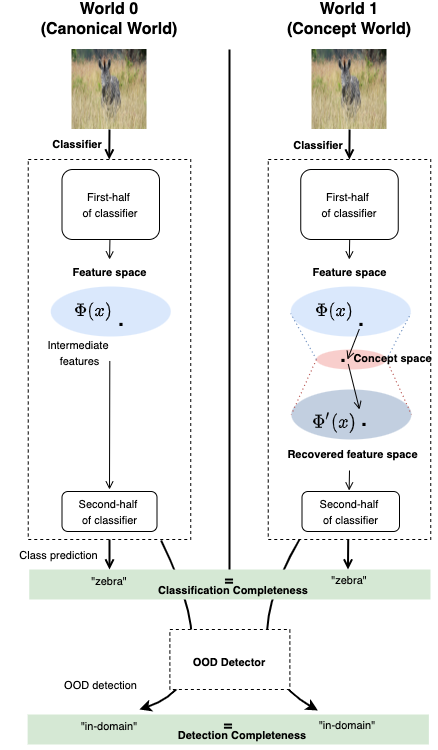
\includegraphics[width=0.45\textwidth]{figures/completeness.png}
% 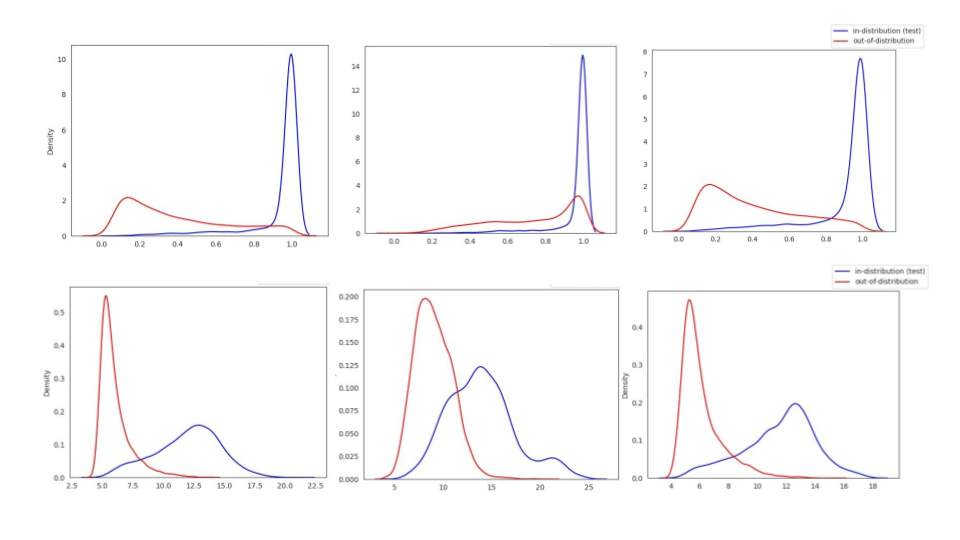
\includegraphics[scale=0.24]{figures/distribution.png}
% %\vspace{-2mm}
% \caption{Blue line is the estimated density of outputs from $\calD$ given ID test data (AwA), and red line is that of OOD test data (SUN). DNN classifier is Inception-V3 trained with AwA dataset.
% \textbf{First row}: distributions of outputs from MSP detector \cite{hendrycks2016msp}. 
% \textbf{Second row}: distributions of outputs from Energy detector \cite{liu2020energy}.
% \textbf{Left}: Target distribution of $S(\bfx, \bff)$ in canonical world. 
% \textbf{Mid}: Distribution of $S(\bfx, \fcon)$ in concept world, using concepts learned by \cite{yeh2019completeness}.
% \textbf{Right}: Distribution of $S(\bfx, \fcon)$ in concept world, using concepts learned by our framework.}
% \vspace{-5mm}
% \label{fig:score-distribution}
% \end{figure}

\begin{figure}[tbp]
\centering
\subfloat[MSP, target \label{fig:distr_msp_target}]{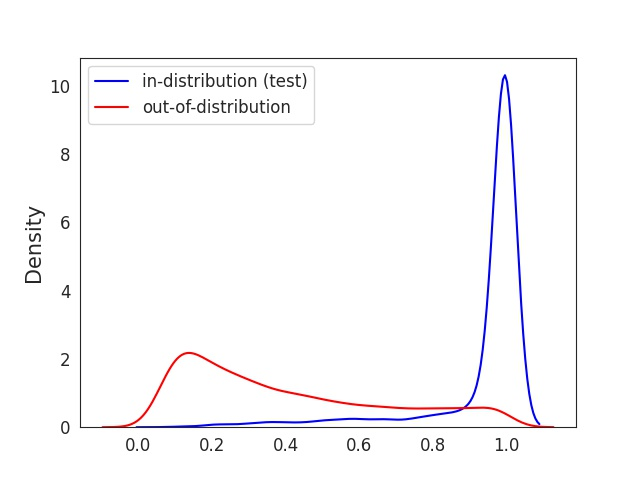
\includegraphics[width=0.15\textwidth]{figures/distr_msp_target.jpg}}\hfill
\subfloat[MSP, baseline \label{fig:distr_msp_yeh}] {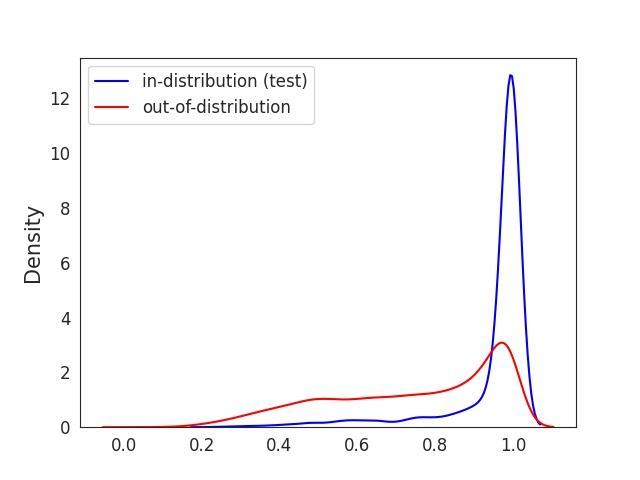
\includegraphics[width=0.15\textwidth]{distr_msp_yeh.jpg}}\hfill
\subfloat[MSP, ours \label{fig:distr_msp_ours}]{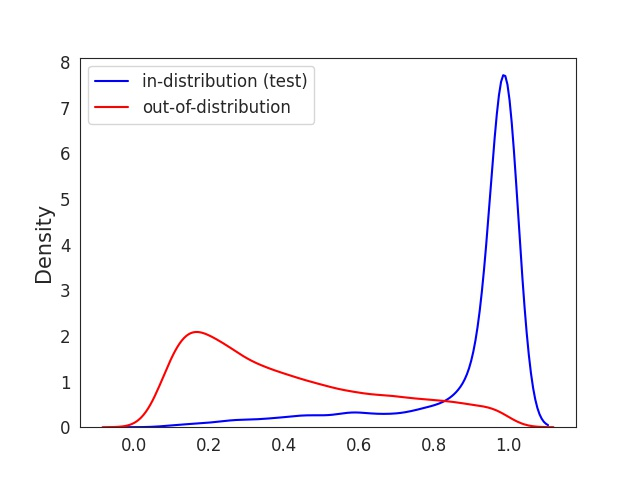
\includegraphics[width=0.15\textwidth]{figures/distr_msp_ours.jpg}} \\
\subfloat[Energy, target\label{fig:distr_energy_target}]{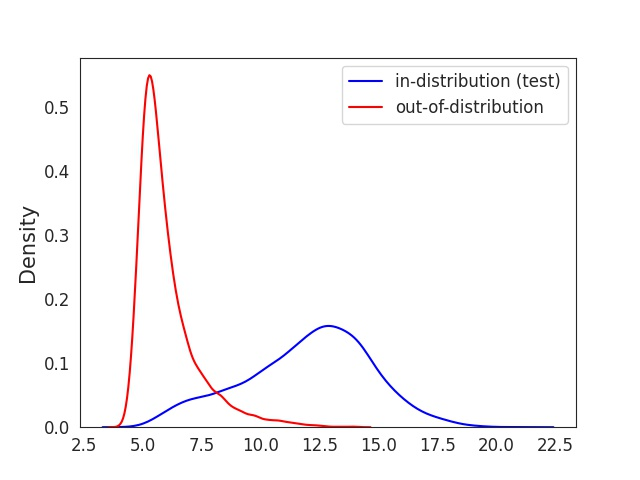
\includegraphics[width=0.15\textwidth]{figures/distr_energy_target.jpg}}\hfill
\subfloat[Energy, baseline \label{fig:distr_energy_yeh}] {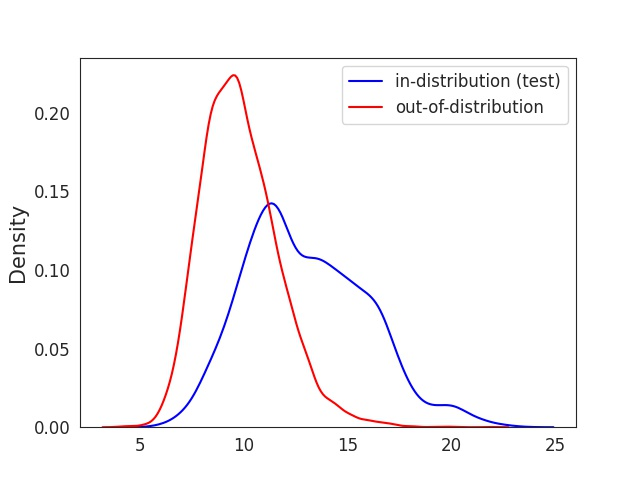
\includegraphics[width=0.15\textwidth]{figures/distr_energy_yeh.jpg}}\hfill
\subfloat[Energy, ours\label{fig:distr_energy_ours}]{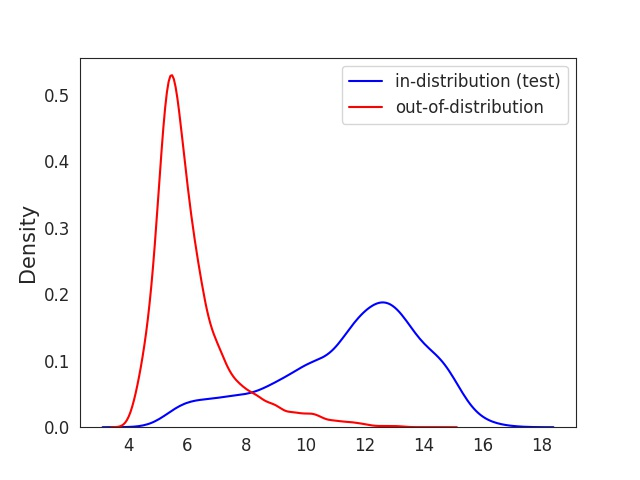
\includegraphics[width=0.15\textwidth]{figures/distr_energy_ours.jpg}}
\caption{Estimated density of $S(\bfx, \cdot)$ between the AwA test data (ID; blue) and the SUN dataset (OOD; red). DNN classifier is Inception-V3 and OOD detector is either MSP \cite{hendrycks2016msp} or \cite{liu2020energy}.
\textbf{Left}: Target distribution of $S(\bfx, \bff)$ in canonical world. 
\textbf{Mid}: Distribution of $\Scon(\bfx, \bff)$ in concept world, using concepts learned by \cite{yeh2019completeness}.
\textbf{Right}: Distribution of $\Scon(\bfx, \bff)$ in concept world, using concepts learned by our method.
For MSP, we set $\lambda_\textrm{mse} = 10, \lambda_\textrm{norm} = 0.1, \lambda_\textrm{sep} = 0$ and for Energy, $\lambda_\textrm{mse} = 1, \lambda_\textrm{norm} = 0.1, \lambda_\textrm{sep} = 0$.}
\label{fig:score-distribution}
\end{figure}

Unfortunately, there is a caveat with their approach.
Eqn. (\ref{equ: baseline}) may encourage the concepts to have high classification completeness score (defined in Eqn. (\ref{equ: completeness-classification})), but their concepts may fail to reduce the gap between canonical world and concept world genuinely. \ryan{By ensuring that they achieve an}
\textit{accurate reconstruction} of $\hat{\calZ}$
, the resulted concept scores would be sufficient enough to recover the accuracy of $\bff$ in expectation, but it is unclear whether the per-instance behavior of $\bff$ (and moreover, $\calD$ that runs based on $\bff$) is genuinely imitated.
To be more specific, $\bfC$ would be a set of $m$ principal vectors 
the set of concept vectors
$m$ unit vectors that fully span the space supported by $\{\bfphi(\bfx_1), \cdots, \bfphi(\bfx_{\Nintr})$.
usually not independent to each other (\eg concept "Greenery" is negatively related to concept "Sea").
have no guarantee on how \textit{accurate} the concepts are in explaining the classifier and the OOD detector.
% The reason we should care about in instance-level behavior of $\bff$ and $\calD$ in concept world is as follows. 
Besides, since the focus of \cite{yeh2019completeness} is initially confined to studying the utility of concepts for classifier with ID data, there is no guarantee for the utility of concepts for OOD detector explanations.

To illustrate with a real example, Figure \ref{fig:score-distribution} shows the distribution of $S(\bfx, \bff)$ and $\Scon(\bfx, \bff)$ on the AwA dataset (ID) and the SUN dataset (OOD).
We observe that $\Scon(\bfx, \bff)$ based on the concepts learned by \cite{yeh2019completeness} has a totally different distribution for OOD data, when compared to the target distribution of $S(\bfx, \bff)$ in canonical world (see Figure \ref{fig:distr_msp_target} and \ref{fig:distr_msp_yeh}).
Not only for OOD data, their concepts result in mismatched distribution of $\Scon(\bfx, \bff)$ also with ID data (see Figure \ref{fig:distr_energy_target} and Figure \ref{fig:distr_energy_yeh}). 
To this end, we propose a general framework for concept learning that complements the previous works by additionally imposing instance-level requirements for concepts, and taking OOD data and OOD detector into consideration.
% \begin{equation}
% \label{equ: baseline+l2}
%     \argmax_{\bfC, g} \, \text{log} \proba_{(\bfx, y) \sim D^{train}_{in}}[\, h_{y}(\hat{\phi}_{g, \bfC}(\bfx))] + \lambda_1 \cdot R_{coherency}(\bfC) + \lambda_2 \cdot
%     \expec_{\bfx \sim D_{train}^{in}}||\phi(\bfx) - \hat{\phi}_{g, \bfC}(\bfx))||_2
% \end{equation}
% \begin{equation}
% \label{equ: baseline+score}
%     \argmax_{\bfC, g} \, \log \proba_{(\bfx, y) \sim D^{train}_{in}}[\, h_{y}(\hat{\phi}_{g, \bfC}(\bfx))] ~+~ \lambda\, R_{coherency}(\bfC) ~-~ \alpha \expec_{\bfx \sim D_{train}^{in}} (\mathcal{D}(h(\hat{\phi}_{g, \bfC}(\bfx))) - \mathcal{D}(f(\bfx)))^2
% \end{equation}

% Let $D^{train} = \{D_{\text{in}}^{train} \cup D_{\text{out}}^{train}\}$, and data is drawn as $(\bfx, s) \sim D^{train}$ where $s \in \{0, 1\}$ is the groundtruth label of OOD detection.
%
% \begin{equation}
% \label{equ: baseline+separability}
%     \argmax_{\bfC, g} \, \log \proba_{(\bfx, y) \sim D^{train}_{in}}[\, h_{y}(\hat{\phi}_{g, \bfC}(\bfx))] ~+~ \lambda\, R_{coherency}(\bfC) ~+~ \beta \expec_{\bfx \sim D^{train}} J(\bfC)
% \end{equation}
%

\begin{algorithm}[t]
\caption{Learning concepts for OOD detector}
\label{alg:concept_learning}
\textbf{INPUT:} Entire training set $\Dtr = \{\Dintr, \Douttr\}$, entire validation set $\Dval = \{\Dinval, \Doutval\}$, classifier $\bff$, detector $\calD$; \\
\textbf{INITIALIZE:} Concept vectors $\bfC = [\bfc_1 ... \bfc_m]$ and parameters of mapping $g$; \\
\textbf{OUTPUT:} $\bfC$ and $g$;
\begin{algorithmic}[1]
  \STATE Identify threshold $\gamma$ for $\calD_\gamma(\bfx, \bff)$ on $\Dval$ at which true positive rate is $95\%$;
%   , and prepare $\widehat{\Dinval}$ and $\widehat{\Doutval}$;
  \FOR{$t = 0, 1, ... T$}
    \STATE Compute prediction accuracy using $\Dintr$ and $\bff$;
    \STATE Compute explainability of $\bfC$ with $\Dintr$ using Eqn. (\ref{equ:regularizer_expl});
	\STATE Compute difference of feature representation between canonical world and concept world using Eqn. (\ref{equ:regularizer_norm});
	\STATE Compute difference of detector outputs between canonical world and concept world using Eqn. (\ref{equ:regularizer_mse});
	\STATE Compute $V_{\textrm{in}}(\bfC)$~\footnotemark and $V_{\textrm{out}}(\bfC)$ using $\Dtr, \calD_\gamma(\cdot)$ and $\bfC$.
	Compute compute separability between $V_{\textrm{in}}(\bfC)$ and $V_{\textrm{out}}(\bfC)$ using Eqn. (\ref{eq:separability_trace}) or Eqn. (\ref{eq:separability_trace_per_class});
    \STATE Update $\bfC$ and $g$ using Eqn. (\ref{equ: concept learning})
  \ENDFOR
\end{algorithmic}
\end{algorithm}
\footnotetext{To make the dimension reduction in $V_{\textrm{in}}(\bfC) := \{\widetilde{v}_{\bfc_i}(\bfx) ~|~ \widetilde{v}_{\bfc_i}(\bfx) = \max_{p, q} |\langle \bfphi^{p,q}(\bfx), \bfc_i \rangle|, \, \bfx \sim \Pin\} $ differential, we take a smooth approximation to the maximum via the \texttt{logsumexp} operation: $\max_{p, q} |\langle \bfphi^{p,q}(\bfx), \bfc_i \rangle| \approx \frac{1}{\alpha}\sum_{p,q}\log(e^{\alpha |\langle \bfphi^{p,q}(\bfx), \bfc_i \rangle|})$ as $\alpha \rightarrow \infty$. The same applies to $V_{\textrm{out}}(\bfC)$.}

\mypara{Concept Learning Objective.}
We suggest a simple design of regularization, inspired by recent works on transferring feature information from the teacher model to the student model \cite{hinton2015distilling,ba2014deep,zhou2018rocket}.
Recall that $\bfC$ projects the space spanned by original feature representations $\calZ$ to concept space, which is then mapped to the reconstructed space $\hat{\calZ}$ by $\bfg$.
Intuitively, to encourage the accurate reconstruction of $\hat{\calZ}$, we require that the distance between $\recphi(\bfx)$ and $\bfphi(\bfx)$ are minimized and push the detector to output\ryan{"and push the detector to output" => "and push towards the detector's output"?}
Hence, we include an additional regularization term that minimizes the squared $\ell_2$ distance between feature representations in $\calZ$ and $\hat{\calZ}$, and the mean squared error between . \jihye{intuition behind using only ID for norm term and usign both ID and OOD for mse term}
\begin{align}
\label{equ:regularizer_norm}
    J_{\textrm{norm}}(\bfC) ~&=~ \expec_{\bfx \sim \Dintr}||\bfphi(\bfx) - \recphi(\bfx)||^2 \\
    \label{equ:regularizer_mse}
    J_{\textrm{mse}}(\bfC) ~&=~ \expec_{\bfx \sim \Dtr} (S(\bfx, \bfh \circ \recphi) - S(\bfx, \bfh \circ \bfphi))^2
\end{align}
\jihye{update to distribution}

Furthermore, to enhance the interpretatbiliy of our concept-based explanations, we impose an additional criterion for the concepts: separability. As already discussed in Section \ref{sec:separability_score}, our proposed separability metric is tractable by gradient-based optimization and can be directly applied to learning objective as a regularization term.
With all regularization terms put together, our final concept learning objective becomes
\begin{align}
\label{equ: concept learning}
\argmax_{\bfC, g}\, &\expec_{(\bfx, y) \sim \Pin}\!\!\big[ \log h_y(\bfg(\VC(\bfx))) \big] ~+~ \lambda_{\textrm{expl}}\, R_{\textrm{expl}}(\bfC) \nonumber \\ 
    &-~ \lambda_{\textrm{mse}}\, J_{\textrm{mse}}(\bfC) ~-~ \lambda_{\textrm{norm}}\,J_{\textrm{norm}}(\bfC) \nonumber \\
    &+~ \lambda_{\textrm{sep}}~J_{\textrm{sep}}(\bfC)
\end{align}
We summarize our complete concept learning algorithm in Algorithm \ref{alg:concept_learning}.



%
% Note that using \begin{align} ... \end{align} is a better way that using \begin{array}
% \begin{equation}
% \label{equ: concept learning}
% \begin{array}{l}
%     \argmax_{\bfC, g} \, \log \proba_{(\bfx, y) \sim D^{train}_{in}}[\, h_{y}(\hat{\phi}_{g, \bfC}(\bfx))] ~+~ \lambda\, R_{coherency}(\bfC) \hspace{20mm} \\
%     -~ \alpha\, \expec_{\bfx \sim D^{train}}\mathcal{D}(h(\hat{\phi}_{g, \bfC}(\bfx))) - \mathcal{D}(f(\bfx)))^2 
%     ~+~ \beta\, \expec_{\bfx \sim D^{train}} J(\bfC) \\
%     -~ \gamma\, \expec_{\bfx \sim D^{train}}||\phi(\bfx) - \hat{\phi}_{g, \bfC}(\bfx))||_2
% \end{array}
% \end{equation}

